\documentclass[a4paper]{article}
\usepackage[utf8]{inputenc}
\usepackage[T1]{fontenc}
\usepackage[french]{babel}
\usepackage{geometry}
\geometry{hmargin=3.5cm,vmargin=3.5cm}
\usepackage{graphicx}
\usepackage[nottoc, notlof, notlot]{tocbibind}

%% \usepackage[vlined, lined, linesnumbered, boxruled, french]{algorithm2e}
\usepackage{fancyhdr}
\pagestyle{fancy}

\lhead{Background}
\rhead{Simulateur de caches multi-c\oe ur}
\lfoot{ENSEIRB-MATMECA}
\rfoot{PFA 2013-2014}

\begin{document}

\thispagestyle{empty}

\vspace{\stretch{1}}
\hrule
\begin{flushleft}
\huge{Simulateur de caches sur\\architecture multi-c\oe ur :}\\
\end{flushleft}
\begin{flushright}
\Huge\textbf{Rapport}\\
\end{flushright}
\hrule

\vspace{\stretch{1}}
\noindent\textbf{Auteurs :}
\emph{DUBOIS Nicolas, GOUDET Pierre, HENG Nicolas, HONORAT Alexandre, MARAIT Gilles, PICHON Grégoire}\\
\\
\noindent\textbf{Client :}
\emph{M. BARTHOU Denis}\\
\\
\noindent\textbf{Responsable pédagogique :}
\emph{M. MORANDAT Floréal} 

\vspace{\stretch{1}}
\normalsize
\begin{center}
  Deuxième année, filière informatique\\
  Date : \today\\
  \textsc{Enseirb-Matmeca}
\end{center}


\newpage
\tableofcontents

\newpage
\section*{Introduction}

\indent Dernièrement la vitesse des processeurs a considérablement augmenté (loi de Moore) alors que le temps d'accès à la mémoire RAM (Random-Access Memory) est resté globalement le même. Pour permettre d'accèder rapidement à des éléments mémoire non contenus dans les registres, des caches sont utilisés. Cette organisation hiérarchique de la mémoire a plusieurs objectifs: \\
\begin{itemize}
\item \^Etre assez conséquente en termes de taille pour pouvoir contenu la totalité de l'espace adressable.
\item \^Etre organisée de manière à être rapide.
\item Ne pas coûter trop cher. \\
\end{itemize}

\indent Les caches permettent de stocker la mémoire utilisée récemment dans les registres, en se basant sur deux concepts: la localité spatiale et la localité temporelle. La localité temporelle stipule qu'une cellule mémoire accédée récemment sera très probablement utilisée dans un futur proche. La localité spatiale est l'idée que si l'on accède à une cellule mémoire $X$, la cellule mémoire $X+1$ a de grandes chances d'être utilisée. \\

\indent Les mémoires de haut niveau, proches du processeur, sont généralement de petite taille. Leur coût est conséquent mais leur accès est très rapide. On peut résumer comme suit une hiérarchie mémoire classique: \\

\begin{figure}[!h]
\begin{center}
   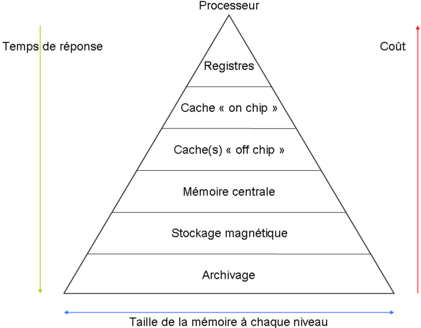
\includegraphics[scale=0.75]{hierarchy.png}
   \caption{\label{hierarchy} Hiérachie mémoire}
\end{center}
\end{figure}

\indent Le but de ce document est de résumer un certains nombre de techniques relatives à la bonne gestion de cette hiérarchie, en se focalisant sur les caches. Nous commencerons par expliciter le comportement d'un cache en général, avant d'étudier les moyens mis en {\oe}uvre afin d'assurer la cohérence de l'ensemble des caches. Nous finirons par proposer quelques algorithmes permettant de simuler de manière la plus générique possible le comportement des caches.

\newpage
\section{Fonctionnement d'un cache}
\indent Cette partie entend préciser le fonctionnement général d'un cache: comment il est possible d'y ajouter une donnée, quelle est la correspondance entre les blocs mémoires et les lignes de cache ou encore comment une donnée peut être evincée d'un cache.

\subsection{\'Etiquettes}
\indent Quand un bloc mémoire (généralement $1$ octet) est ajouté dans le cache, la ligne entière correspondante ($32$ ou $64$ octets) est chargée dans le cache, afin d'exploiter le principe de localité spatiale et de faire du prefetching de données. Pour pouvoir retrouver une donnée dans le cache, une table d'étiquettes est tenue à jour. Concrètement, une adresse mémoire est séparée en trois champs comme sur la figure suivante: \\

\begin{figure}[!h]
\begin{center}
   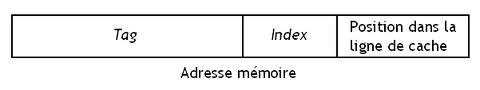
\includegraphics[scale=0.50]{etiquette.jpeg}
   \caption{\label{etiquette} Adresse mémoire}
\end{center}
\end{figure}

\indent Le tag est stocké dans la table des étiquettes, il servira a identifier les différents blocs mémoires pouvant être au même endroit dans un cache. L'index correspond au numéro de set dans lequel se trouve la ligne de cache. Pour finir l'offset correspond au bloc dans la ligne de cache.

\subsection{Fonction de correspondance}
\indent Un cache de taille $n$ contient un ensemble $p$ de lignes de taille $m$, tels que $n = p \times m$. Afin de placer et récupérer une donnée dans le cache, une fonction de correspondance avec la mémoire est nécessaire. Il existe trois cas de figure. Pour la suite, nous prendrons: \\
\begin{itemize}
\item $i$ le numéro de set du cache
\item $j$ le numéro du bloc mémoire
\item $s$ le nombre de sets du cache
\item $k$ l'associativité du cache 
\end{itemize}

\subsubsection{Direct associative}
\indent Un cache est en correspondance directe si à chaque bloc mémoire est associé une unique ligne du cache. Le nombre de sets, $s$, du cache est alors égal à son nombre de lignes, $p$. Lorsqu'un bloc mémoire $j$ est ajouté dans le cache, la ligne correpondante est chargée à la ligne $i = j\ modulo\ s$. Avec ce type de cache, il est facile d'ajouter ou de retrouver une données. Cependant, si plusieurs blocs mémoires correpondant à la même ligne de cache sont fréquemment utilisés, il faudra sans cesse supprimer et ajouter des données dans le cache.

\subsubsection{Fully associative}
\indent Un cache est en correspondance associative si chaque bloc mémoire peut être mis dans n'importe quelle ligne du cache. Il n'y a alors qu'un seul set. L'inconvénient précédent n'est plus existant, cependant il devient beaucoup plus compliqué de rechercher une donnée dans le cache. L'ensemble des tags doit en effet être parcouru.

\subsubsection{$k$-ways associative}
\indent Les deux cas présentés précedemment présentent des inconvénients. Généralement, un cache profite des avantages des deux visions en faisant un compromis. Dans le cas de la correspondance associative par ensemble, chaque set possède un nombre $k$ de lignes, appelé associativité du cache et tel que $p=k \times s$. La fonction de correspondance est telle que $i = j\ modulo\ s$. De cette manière, un bloc mémoire peut se trouver dans un ensemble de $k$ lignes. Il est donc possible d'avoir plusieurs blocs mémoires correspondant au même ensemble sans trop perdre en performances et l'algorithme de recherche est plus efficace que dans le cas de la correspondance associative.

\subsection{Politiques de remplacement}


\newpage
\section{Gestion de la cohérence}

\subsection{Présentation du problème}

\subsection{Protocoles de cohérence}


\newpage
\section{Fonctionnement global}

\subsection{Caches inclusifs}

\subsection{Caches exclusifs}

\subsection{Caches non-inclusifs}


\newpage
\section{Comportements spéciaux}

\subsection{Utilisation d'un victim cache}

\subsection{Tracking}


\newpage
\section{Algorithmes de simulation}

\subsection{Interaction entre les différents niveaux de caches}

\subsection{Gestion des différentes modularités}

\newpage
\nocite{*}
\bibliographystyle{plain}
\bibliography{rapport}

\end{document}
